\documentclass[conference]{IEEEtran}
\IEEEoverridecommandlockouts
% The preceding line is only needed to identify funding in the first footnote. If that is unneeded, please comment it out.
\usepackage{cite}
\usepackage{amsmath,amssymb,amsfonts}
\usepackage{algorithmic}
\usepackage{graphicx}
\usepackage{textcomp}
\usepackage{overpic}
\usepackage{xcolor}
\usepackage{hyperref}
\def\BibTeX{{\rm B\kern-.05em{\sc i\kern-.025em b}\kern-.08em
    T\kern-.1667em\lower.7ex\hbox{E}\kern-.125emX}}
\newcommand\todo[1]{\textcolor{red}{TODO #1}}

\begin{document}

\title{Virtual Neurorobotics in the Human Brain Project}
\author{Max Becker, Olivier Boder and Qianlin Wu\\FZI Forschungszentrum Informatik\\Karlsruhe, Germany}

\maketitle

\begin{abstract}

\end{abstract}

\begin{IEEEkeywords}
Spiking Neural Networks, Evolutionary Algorithms, Neurorobotics Platform, Human Brain Project
\end{IEEEkeywords}


% !TEX root = ../Ausarbeitung.tex
\section{Introduction}
\label{sec:intro}
In scope of the \textit{Praktikum} within the Human Brain Project, we work with the Neurorobotics Platform (NRP) which provides a simulation environment for robotics.
More specifically, our experiment setup consists of a table, on which a robot arm is placed.
The robot arm has six joints and a hand with five fingers.
In front of the robot arm, a cylinder is placed on the table.
The goal of the Praktikum is to move the cylinder as far as possible with the robot arm.
This can be performed by just hitting the cylinder away or by grabbing the cylinder and throwing it as far as possible.
The performance is measured by the distance of the cylinder from the table.
The setup is depicted in \autoref{fig:hbbprak_2018}.

In the following, several strategies to fulfill this task are presented.
To begin with, fundamentals of evolutionary algorithms and spiking neural network are explained in \autoref{sec:ea} respectively \autoref{sec:spiking}.
Subsequently, a hard-coded approach in \autoref{sec:hard-coded} followed by a more sophisticated learning approach with evolutionary algorithms in \autoref{sec:learned} are presented to solve the challenge.
Then, \autoref{sec:problems} depicts some obstacles that arose during the experiments and the Praktikum.
Finally, the results are presented in \autoref{sec:results} and a conclusion is drawn in \autoref{sec:conclusion}

\begin{figure}[h]
\centering
\includegraphics[width=.95\columnwidth]{figures/hbpprak_2018.png}
\caption{The goal is to throw the cylinder as far as possible.}
\label{fig:hbbprak_2018}
\end{figure}
% !TEX root = ../Ausarbeitung.tex
\section{Evolutionary Algorithms}
\label{sec:ea}
Evolutionary algorithms are inspired by nature and evolution.
They try to approximate a solution following the principle of survival of the fittest.
In fact, an evolutionary algorithm models a population consisting of several individuals performing a task, such as an optimization problem, and are evaluated by a fitness function.
One of these populations is called a generation.
The elite of each generation, i.e. the individuals performing best according to their fitness, is then selected to evolve the next generation.
This allows the population to evolve towards a solution.
The evolution of a population corresponds to the mutation of individuals.
The evolution process is depicted in \autoref{fig:ea}.

\begin{figure}[h]
\centering
\includegraphics[width=.7\columnwidth]{figures/ea_fig.pdf}
\caption{An illustration of an evolutionary algorithm learning.}
\label{fig:ea}
\end{figure}

To mutate a population, the crossover strategy can be applied.
Crossover is used to generate new offspring by combining genetic information of two parents.
One way to combine their genetic information is single-point crossover.
A point is randomly picked on the genetic sequence, where it is separated at the same point of both parents.
The second part, i.e. the tail, is then swapped between the parents.
Hence, each parent has its own genetic information until the chosen point, following by the genetic sequence of the other parent.
To apply more variety into the recombination of the genetic information k-point crossover can be applied.
Instead of only one point, more such random points are picked in the sequence, at which alternately information is swapped between the parents.

As individuals are evolving over generations, they may improve their fitness and thus optimize a solution for the task.
Their genetic information can therefore be parameters to solve a problem.
Overall, there is no specific or correct parameter assumption needed for initialization, as they will be approximated by evolving over generations.

% !TEX root = ../Ausarbeitung.tex
\section{Spiking Neural Networks}
\label{sec:spiking}
Spiking neural networks try to mimic natural neural networks more closely than other artificial neural networks.
The neurons in spiking neural networks are connected via synapses which are weighted and organised in a directed graph.
Every neuron in the network has a membrane potential.
If this potential exceeds a certain threshold, the neuron fires, meaning it sends a spike to all its succeeding neurons in the network.
The potential of the spiking neuron is then reset and, depending on the implementation, the neuron may enter a short refractory period in which it cannot fire again.
If a neuron receives a spike from a predecessor, its membrane potential rises or falls depending on the synapse being inhibitory or excitatory.
In the periods between spikes, the neurons leek some of their potential\cite{b1}.

To learn with spiking neural networks, the weights of the synapses have to be changed.
These weights determine how much influence a spike has on the potential of a succeeding neuron.
In contrast to other artificial neural networks, the neurons don't have to be organized in strict layers and not all neurons in a layer need to be computed at the same time.
The information is less encoded in the neurons values and more in the timing of the spikes\cite{b2}.
However, it is harder to learn with spiking neural networks, because the spikes aren't differentiable, which means the weights cannot be learned using error backpropagation.
One possibility to learn the weights are evolutionary algorithms.

Spiking neural networks are a good option for robot controlling tasks as they try to simulate biological neural networks as similarly as possible and offer advantages in speed, energy efficiency and computation capabilities\cite{b3}.

\section{Hard-coded Approach}
\label{sec:hard-coded}
The tasks of "Hard-code Approach" involves mainly about defining various states for the robot, giving parameters empirically for each state, and trying to grab Cylinder anywhere on the table.In this case the evolutionary algorithm does not need to consider how to optimize the order of the various states and the duration of each state but only needs to optimize the motion parameters in each state. So that it can get a relatively better effect in a shorter time.

\subsection{State Machine}

Such as the picture shown in \autoref{fig:statemachine} there are 5 states in state mashine, and they communicate with 2 control interface: Arm Control and Hand Control.These states: Approach, Prepare, Throw give Arm Control commands(string typ) via ROS, and states: Grasp, Release give Hand Control. In these two Control Interfase , each instruction corresponds to parameters for the control of robot.These parameters were originally obtained empirically and then optimized by evolutionary algorithms later. 

The state of Throw and Release was originally designed to execute Release state after Throw state has been executed for a short time, in order to get a farther throw distance.But because of the bug of model, this will break the entire simulation.So these two states can only be executed at the some time. 

\begin{figure}[htpb]
\centering
	\includegraphics[width=0.96\linewidth]{figures/state.pdf} 
	\caption{State and Control Interface}
	\vspace{-0.4cm}
	\label{fig:statemachine}
\end{figure}

\subsection{Inverse Kinematics}

The ability to grab a cylinder anywhere on the table is achieved by inverse Kinematic. Because the camera in the model cannot get the depth value of the object, its coordinates are not available through the camera. So as a simplification, when the cylinder is generated, its world coordinates are immediately posted to a topic. As the picture shown in \autoref{fig:top},we assume that the cylinder posion ist $(C_x, C_y, C_z)$, and the robitic origin position is  $(R_x, R_y, R_z)$, so the amr1 move configution $M_1$ can be caculate with the equation below:


\begin{equation}
\label{simple_equation}
M_1=\alpha = arctan((C_y-R_y)/(C_x-R_x))
\end{equation}









\begin{figure}[htpb]
\centering
	\includegraphics[width=0.96\linewidth]{figures/top_view.pdf} 
	\caption{Platform top view}
	\vspace{-0.4cm}
	\label{fig:top}
\end{figure}


The \autoref{fig:right} show the look of the model from the right side. Since there is already a perfect configution that makes the robot close to the cylinder(that means $\beta$ and $\gamma$ is known).So the lengs of arm2: a and arm4: b can be caculated with:

\begin{equation}
\begin{aligned}
a=c*sin(\gamma)/sin(\delta)\\b=c*sin(\beta)/sin(\delta)\\ 
\textbf{with}\ c=\sqrt{(R_x-C_x)^2+(R_y-C_y)^2}\\\delta=2*\pi-\beta-\gamma.
\end{aligned}
\end{equation}



When the cylinder is created anywhere on the table, the move configuration of arm2:$M_2$ amr4: $M_4$, arm6: $M_6$ can be caculate with equation below since amr1 and arm4 lengs are known.The move configutions for arm3, amr5 remain the same as before. 
 


\begin{equation}
\begin{aligned}
M_2=\beta=arccos((a^2+c^2-b^2)/2*a*c)\\
M_4=\pi-\delta=\pi-arccos((a^2+b^2-c^2)/2*a*b)\\
M_6=\gamma=arccos((b^2+c^2-a^2)/2*b*c)\\
\textbf{with}\ c=\sqrt{(R_x-C_x)^2+(R_y-C_y)^2}
\end{aligned}
\end{equation}

\begin{figure}[tpb]
\centering
	\includegraphics[width=0.96\linewidth]{figures/right_v.pdf} 
	\caption{Platform right view}
	\vspace{-0.4cm}
	\label{fig:right}
\end{figure}




% !TEX root = ../Ausarbeitung.tex
\section{Learned Approaches}
The next approach was trying to learn some of the movements instead of hard-coding them.
We used an evolutionary approach to learn weights for a spiking neural network which controls the robots movements.

\subsection{Evolutionary Approach}
In this approach the robot is controlled by a spiking neural network which can be seen in \autoref{fig:network}.
The network has three input and seven output neurons which are fully connected.
The three dimensional position of the cylinder is used for the input neurons.
Six of the output neurons control the six joints of the robots arm and the last neuron controls when the hand should release the cylinder.

The individuals of our evolutionary algorithm are lists of 21 values each representing one weight of the network.
To evaluate the individuals a throw is simulated and the distance of the cylinder from the table represents the fitness of the individual.
After each individual of a generation is evaluated we select the elite which consists of the best 50\% of the individuals.
The elite gets copied into the next generation and the remaining individuals are generated by mutating the individuals of the elite.

\begin{figure}[h]
\centering
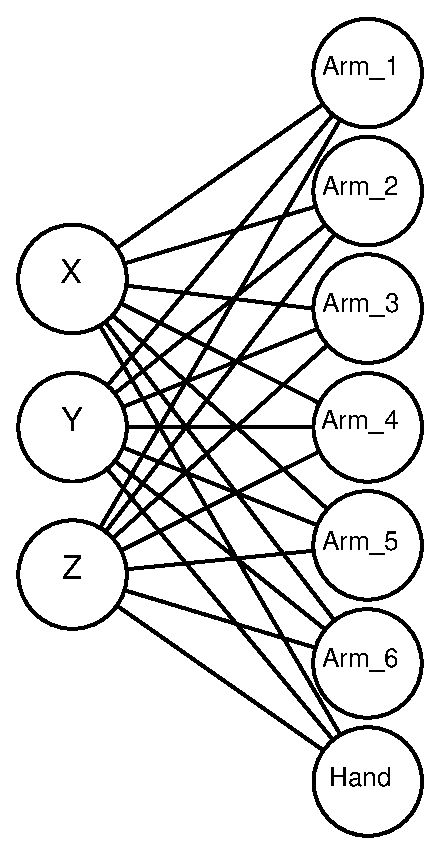
\includegraphics[width=.5\columnwidth]{figures/net.eps}
\caption{Network architecture.}
\label{fig:network}
\end{figure}

\subsubsection{Mutation Strategies}
Three different mutation strategies were implemented to generate new descendants.
The first method uses only one parent and adds or subtracts small random values from its weights.
The other two methods use two parents.
One was a single-point crossover at a random position meaning you take the first n weights from one parent and the remaining ones from the second one.
The last method is a k-point crossover.
At each position this method chooses randomly one of the parents weights.

\subsection{Simplified Problem}
As our first learned approach wasn't really successful we try to reduce the search space for the evolutionary algorithm.
To achieve this we restrict which joints the robot could use to execute the throw.
We fix all rotational joints by setting the respective weights in the neural network to zero because this probably won't impact the robots ability to make a good throw very much.
This reduces the number of weights to be learned from 21 to 12.
\section{Problems}\label{problems}

\todo{}

\section{Results}
We enabled the robot to grasp the cylinder at random positions and throw it with a set of synaptic weights generated by the evolutionary algorithm.
However the problems described in section \ref{problems} made it very hard to learn anything.
The individuals of the evolutionary algorithm executed throws but due to non-deterministic behaviour of the simulation the measured distance sometimes differed a lot from the quality of the movement.
The non-determinism also made it hard to compare the results as the same individual gets different distances if you execute it multiple times.
That resulted in the algorithm not really learning anything and evolving the weights rather randomly.
\todo{}
% !TEX root = ../Ausarbeitung.tex
\section{Conclusion}
\label{sec:conclusion}
\todo{}
Two different approaches are presented to make the robot arm throwing the cylinder.
The first approach controls the robot arm with hard-coded configurations which have been determined empirically.
This not only involves the static movements of the robot, but also grasping the cylinder at random positions reliably which is computed with inverse kinematics.
The second approach aims for a learned solution based on spiking neural networks.
For this purpose, an evolutionary algorithm has been chosen in order to optimize the synaptic weights.
Given the circumstances, various approaches have been implemented that lead to reasonably results.
However, results are not comparable due to non-deterministic behavior.

\subsection{Future Work} % (fold)
\label{sub:future_work}
\todo{}

% subsection future_work (end)



\begin{thebibliography}{00}
\bibitem{b1} G. Eason, B. Noble, and I. N. Sneddon, ``On certain integrals of Lipschitz-Hankel type involving products of Bessel functions,'' Phil. Trans. Roy. Soc. London, vol. A247, pp. 529--551, April 1955.
\end{thebibliography}


\end{document}
